%%%%%%%%%%%%%%%%%%%%%%%%%%%%%%%%%%%%%%%%%%%%%%%%%%%%%%%%%%%%%%%%%%%%%
% Use the koma-script document style
%\documentclass{scrbook}
%\KOMAoptions{twoside=false} % disable two-side formatting for scrbook
% alternatively, for shorter essay, use the following
\documentclass{scrartcl}
%%%%%%%%%%%%%%%%%%%%%%%%%%%%%%%%%%%%%%%%%%%%%%%%%%%%%%%%%%%%%%%%%%%%%

%%%%%%%%%%%%%%%%%%%%%%%%%%%%%%%%%%%%%%%%%%%%%%%%%%%%%%%%%%%%%%%%%%%%%
% Useful packages
\usepackage{mathtools}
\usepackage{amssymb,bm,bbold}
\usepackage[colorlinks=true]{hyperref}
\usepackage{enumerate}

\usepackage{fullpage}

\usepackage[font=scriptsize,labelfont=bf]{caption}
\usepackage{wrapfig}
\usepackage{tikz}
\usepackage{pgfplots}

\usepackage[]{natbib}
\bibliographystyle{chicago}

%=================================
% pre-defined theorem environments
\usepackage{amsthm}
\newtheorem{theorem}{Theorem}
\newtheorem{lemma}{Lemma}
\newtheorem{proposition}{Proposition}
\newtheorem{corollary}{Corollary}
\newtheorem{definition}{Definition}
\newtheorem*{remark}{Remark}
\newtheorem*{assumption}{Assumption}

\usepackage[framemethod=tikz]{mdframed}
\newmdtheoremenv[
skipabove=\baselineskip,
skipbelow=\baselineskip,
hidealllines=true,
innertopmargin=4pt,
linewidth=4pt,
linecolor=gray!40,
singleextra={
  \draw[line width=3pt,gray!50,line cap=rect] (O|-P) -- +(1cm,0pt);
  \draw[line width=3pt,gray!50,line cap=rect] (O|-P) -- +(0pt,-1cm);
  \draw[line width=3pt,gray!50,line cap=rect] (O-|P) -- +(-1cm,0pt);
  \draw[line width=3pt,gray!50,line cap=rect] (O-|P) -- +(0pt,1cm);
  },
firstextra={
  \draw[line width=3pt,gray!50,line cap=rect] (O|-P) -- +(1cm,0pt);
  \draw[line width=3pt,gray!50,line cap=rect] (O|-P) -- +(0pt,-1cm);
},
secondextra={
  \draw[line width=3pt,gray!50,line cap=rect] (O-|P) -- +(-1cm,0pt);
  \draw[line width=3pt,gray!50,line cap=rect] (O-|P) -- +(0pt,1cm);
}
]{problem}{Problem}

%=================================
% useful commands
\DeclareMathOperator*{\argmin}{arg\,min}
\DeclareMathOperator*{\argmax}{arg\,max}
\DeclareMathOperator*{\supp}{supp}
\DeclareMathOperator*{\minimize}{\mathsf{minimize}}

\def\vec#1{{\ensuremath{\bm{{#1}}}}}
\def\mat#1{\vec{#1}}

%=================================
% convenient notations
\newcommand{\XX}{\mathbb{X}}
\newcommand{\RR}{\mathbb{R}}
\newcommand{\EE}{\mathbb{E}}
\newcommand{\PP}{\mathbb{P}}

\newcommand{\sB}{\mathcal{B}}
\newcommand{\sK}{\mathcal{K}}
\newcommand{\sL}{\mathcal{L}}
\newcommand{\sX}{\mathcal{X}}

\newcommand{\TODO}{\textbf{\textsf{TODO}}}

\usepackage{algpseudocode}
\usepackage{algorithm}

%%%%%%%%%%%%%%%%%%%%%%%%%%%%%%%%%%%%%%%%%%%%%%%%%%%%%%%%%%%%%%%%%%%%%
% Typography, change document font
%\usepackage[libertine,cmintegrals,cmbraces,vvarbb]{newtxmath}
%\usepackage[scaled=0.95]{inconsolata}
\usepackage{lmodern}
\usepackage{charter}
\usepackage[scaled=0.95]{inconsolata}

\title{Intuitions for Convex Optimization}
\author{pluskid}

\begin{document}
\maketitle
\tableofcontents

\section*{Preface}
Originally I wanted to write down some notes of the intuitions I developed when trying to
understand various optimization algorithms. Gradually I realized it becomes very difficult to
organize the contents in a coherent way. Since \citet {MAL-050} is an excellent book (and the main
reference here) that already includes most of the topics that I wanted to cover in this notes. I
decided to follow the organization in that book and fill in my thoughts and notes accordingly. The
original book is available at \href{http://www.princeton.edu/~sbubeck/}{S{\'e}bastien Bubeck's
homepage}.

\section{Introduction}
\section{Convex optimization in finite dimension}
\section{Dimension-free convex optimization}
In this chapter, we study the basic gradient descent algorithm and its variants. This algorithm only
requires a first-order oracle that evaluates the gradient (or subgradient) at a given point. The
convergence rate can be characterized in the number of oracle calls, which is remarkably independent
of the input dimension\footnote{Although as also noted in the book, the computational complexity
remains at least linear in the dimension since we need to manipulate the gradient vector. Moreover,
the constants (Lipschitz constant or radius of the feasible parameters) usually depend on the
dimension when we consider specific problems in, machine learning, for example.}. In many cases,
evaluating the first order oracle involves only the same computational complexity as evaluating the
function itself (e.g. the loss function for learning a structured SVM).

\begin{remark}[Lemma 3.1]
This lemma will be useful when we consider constrained optimization where a projection is usually
used in each iteration to make sure the parameters remain feasible. In particular, this lemma shows
that projection onto a convex set $\sX$ is a \emph{contraction}:
\begin{equation}
  \|\Pi_\sX(x)-\Pi_\sX(x')\| \leq \|x-x'\|
\end{equation}
The inequality can be easily shown by applying Lemma 3.1:
\[
  \begin{aligned}
  \|x-x'\|^2
  &= \|x-\Pi_\sX(x) + \Pi_\sX(x)-\Pi_\sX(x') + \Pi_\sX(x') - x'\|^2 \\
  &= \|\Pi_\sX(x)-\Pi_\sX(x')\|^2 + \|x-\Pi_\sX(x)\|^2 + \|x'-\Pi_\sX(x')\|^2 \\
  &\mathrel{\phantom{=}}
     + 2\langle x-\Pi_\sX(x), \Pi_\sX(x)-\Pi_\sX(x')\rangle
     + 2\langle \Pi_\sX(x)-\Pi_\sX(x'), \Pi_\sX(x')-x'\rangle \\
  &\mathrel{\phantom{=}}
     + 2\langle x-\Pi_\sX(x), \Pi_\sX(x')-x'\rangle \\
  &\geq \|\Pi_\sX(x)-\Pi_\sX(x')\|^2 + \|x-\Pi_\sX(x)\|^2 + \|x'-\Pi_\sX(x')\|^2 \\
  &\mathrel{\phantom{=}}
     + 2\langle x-\Pi_\sX(x), \Pi_\sX(x')-x'\rangle \\
  &= \|\Pi_\sX(x)-\Pi_\sX(x')\|^2 + \|(x-\Pi_\sX(x)) + (\Pi_\sX(x')-x')\|^2 \\
  &\geq \|\Pi_\sX(x)-\Pi_\sX(x')\|^2
  \end{aligned}
\]
\end{remark}

\subsection{Projected subgradient descent for Lipschitz functions}

\begin{figure}
\centering
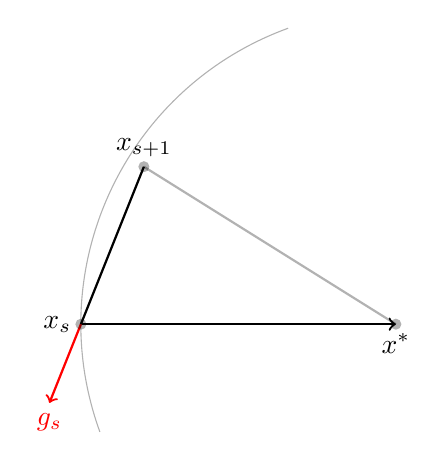
\begin{tikzpicture}[scale=2.0]
  \coordinate [label=left:$x_s$] (Xt) at (-2,0);
  \coordinate [label=below:$x^*$] (Xs) at (0,0);
  \coordinate [label=above:$x_{s+1}$] (Xtp) at (-1.6,1);
  \draw [->,thick] (Xt) -- (Xs);
  \draw [thick] (Xt) -- (Xtp);
  \draw [thick,opacity=.3] (Xs) -- (Xtp);
  \draw [->,thick,red] (Xt) -- (-2.2,-0.5) node [below] {$g_s$};

  \fill [black,opacity=.3] (Xt) circle (1pt);
  \fill [black,opacity=.3] (Xtp) circle (1pt);
  \fill [black,opacity=.3] (Xs) circle (1pt);
  \draw [opacity=.3] ([shift=(110:2)] 0,0) arc (110:200:2);
\end{tikzpicture}
\caption{Demonstration of subgradient descent.}
\label{fig:subgrad-descent-demo}
\end{figure}

\begin{remark}[Theorem 3.2]
The intuition behind the proof is that by the property of subgradient,
\begin{equation}
  0\leq f(x_s) - f(x^*) \leq g_s^\top (x_s-x^*) = -g_s^\top (x^*-x_s)
  \label{eq:subgrad-lower-bound-f}
\end{equation}
where the left hand side is due to the optimality of $x^*$. This inequality indicates that the
vector $x^*-x_s$ is non-negatively correlated with $-g_s$, the direction of a subgradient descent.

Unlike in the case of differentiable functions, in which we can guarantee that the function values
decreases when moving along the direction of negative gradient with a small enough step size; here
we do not know much about the function values. But as we can see from Figure~\ref
{fig:subgrad-descent-demo}, when the angle between $-g_s$ and $x^*-x_s$ is greater than or equal to
$\pi/2$, we will move away from $x^*$ with any positive step size. However, if $f(x_s)-f(x^*)>0$,
i.e. we are not already at the optimal, the angle is strictly less than $\pi/2$, so if we move with
a ``small enough'' step size, we will get closer to $x^*$. Algebraically,
\begin{equation}
\begin{aligned}
  \|x_{s+1}-x^*\|^2 &\leq \|y_{s+1}-x^*\|^2 = \|y_{s+1}-x_s + x_s-x^*\|^2 \\
  &= \eta_s^2\|g_s\|^2 + \|x_s-x^*\|^2 - 2\eta_sg_s^\top (x_s-x^*) \\
  &\leq {\color{red}\eta_s^2\|g_s\|^2} + \|x_s-x^*\|^2 - {\color{blue}2\eta_s\left(f(x_s)-f
  (x^*)\right)}
  \label{eq:subgrad-lipschitz-analysis-step}
\end{aligned}
\end{equation}
Since $\|g_s\|\leq L$ by our assumption, the \textcolor{red}{red term} decays quadratically as
$\eta_t\rightarrow 0$, while
the \textcolor{blue}{blue term} only decays linearly. So when $\eta_s$ is small enough, we will have
$\|x_{s+1}-x^*\|^2 \leq \|x_s-x^*\|^2$. Furthermore, the progress we make by moving towards $x^*$ is
characterized by $f(x_s)-f(x^*)$. So if we are still far away from the optimal, we will be making
quite a lot progress in each step. On the other hand, when $f(x_s)-f(x^*)$ is small, our progress
might be small, but at that point we are already close to the optimal function value $f(x^*)$.

Actually, to get a bound on the algorithm, we can just sum up the previous inequality for all
$s=0,\ldots,t-1$,
\[
  \begin{aligned}
    0\leq\|x_t-x^*\|^2
    &\leq \|x_0-x^*\|^2 + \sum_{s=0}^{t-1}\eta_s^2\|g_s\|^2 - 2\sum_{s=0}^{t-1}\eta_s \left(f(x_s)-f
    (x^*)\right) \\
    &\leq R^2 + L^2\sum_{s=0}^{t-1}\eta_s^2 -2\left(\min_{0\leq s\leq t}f(x_s) - f
    (x^*)\right)\sum_{s=0}^{t-1}\eta_s
  \end{aligned}
\]
It then implies
\begin{equation}
\min_{0\leq s\leq t}f(x_s) - f(x^*)
\leq \frac{R^2 + L^2\sum_{s=0}^{t-1}\eta_s^2}{2\sum_{s=0}^ {t-1}\eta_s}
\label{eq:subgrad-descent-convergence-0}
\end{equation}
\end{remark}

\subsubsection*{Theorem assumptions}
This theorem deals with almost the most general case: the function is
assumed to be convex but not necessarily differentiable. Several minimum assumptions are still
needed for both the algorithm and convergence rate.

Firstly, it is assumed that $\sX\subset \sB(0; R)$. This quantity is mostly to characterize how far
the initial guess is from the optimal solution. The step size will also depend on (proportional to)
the radius $R$: intuitively, if $R$ is too large, using relatively too small step sizes will take a
long time to converge.

The second assumption is the $L$-Lipschitzness of $f$.Since $f$ is convex know that $x^*$ is a
minimizer of $f$ if and only if $0\in\partial f (x^*)$. However, without making any extra
assumptions, we have no idea of the behavior of $f$ even in a small neighborhood of $x^*$. Consider
for example $f(x)=C|x|$, with $C>0$ a large constant. Assume we are currently very close to the
optimal $x^*=0$, say $x_s=\varepsilon$, $\varepsilon>0$. $f$ is differentiable at $\varepsilon$, so
the only subgradient is $g_s=C$. Therefore,
\[
  x_{s+1} = x_s - \eta_s g_s
  = \varepsilon - \eta_sC < -\varepsilon, \quad \forall \eta_s > \frac {2\varepsilon} {C}
\]
As we can see, unless the stepsize $\eta_s$ is very tiny, we will overshoot, $f(x_{s+1})>f(x_s)$.
Moreover, if we use a constant stepsize $\eta_s=\eta$. Then if $\eta >\varepsilon/C$, we will be
jumping back and forth at $\varepsilon$ and $\varepsilon - \eta C$, not able to make any further
progress.

In order to fix this, we need to make additional assumptions. In the case of
smooth functions, the gradient changes continuously. So we know that at a local neighborhood of the
optimal (gradient is 0), the gradient is also small. But here, we are working with
non-differentiable functions, so we will just assume $f$ is $L$-Lipschitz.

Note $f$ being $L$-Lipschitz in $\sX$ implies that $\|g\| \leq L$, $\forall g\in\partial f(x),
\forall x\in\sX$. Knowing an upper bound of $\|g\|$, we could then choose a small enough (according
to $L$) step size to avoid overshooting. This choice guarantees convergence, but tiny step size is
also the source of the slow convergence of subgradient descent algorithms.

Both $R$ and $L$ can typically be estimated for real world problems. Estimating does not need to be
exact, loose upper bounds will still have the convergence guarantee, but the convergence will be
slower.

\subsubsection*{Choosing the step size}
The text after the theorem mentioned that the step size depending on the total number of iterations
$t$ is a bit strange --- if I want to run the algorithm for more iterations, I will have to start
over from scratch with a different step size. Using non-constant decaying step sizes independent of
$t$ is actually possible.

We first describe how the ``magic'' step size in Theorem 3.2 $\eta=R/(L\sqrt{t})$ is chosen, and
then generalize it to decaying step sizes.
Note \eqref{eq:subgrad-descent-convergence-0} holds for any choices of step sizes $\eta_s$ (though
some of them will give completely trivial bounds). So we could actually optimize the right hand side
to get an ``optimal'' bound. To make the problem easier, we choose a fixed stepsize $\eta_s=\eta$
for $s=0,\ldots,t-1$. So the right hand side becomes
\begin{equation}
  \frac{R^2+L^2t\eta^2}{2t\eta} = \frac{R^2}{2t\eta} + \frac{L^2\eta}{2} \geq \frac{LR}{\sqrt{t}}
  \label{eq:subgrad-bound-fix-eta}
\end{equation}
where the inequality holds with equality when
\begin{equation}
  \eta = \frac{R}{L\sqrt{t}}
\end{equation}
The dependency of $\eta$ on $R$ and $L$ is described in the remarks about Theorem assumptions. The
dependency on $t$ is also intuitive: if we have a larger time budget, we can be a little bit more
careful and move slowly.

In general, we can also use a decaying learning rate. Specifically, as long as
$\sum_s\eta_s\rightarrow \infty$ and $\sum_s\eta_s^2$ is bounded or approaches infinity at a slower
rate than $\sum_s\eta_s$, \eqref{eq:subgrad-descent-convergence-0} will give a reasonable bound. For
example, take $\eta_s=R/(L\sqrt{s+1})$, since
\[
\begin{aligned}
  \sum_{s=0}^{t-1} \frac{1}{s+1} &\leq 1 + \int_1^{t} \frac{1}{x}\,dx = 1 + \log t \\
  \sum_{s=0}^{t-1} \frac{1}{\sqrt{s+1}} &\geq \int_1^{t+1}\frac{1} {\sqrt{x}}\,dx =
  2\sqrt{t+1}-2
\end{aligned}
\]
Plug-in to \eqref{eq:subgrad-descent-convergence-0}, we get
\begin{equation}
  \min_{0\leq s \leq t} f(x^s) - f(x^*)
  \leq LR \frac{1+\log t}{4\sqrt{t+1}-4} \lesssim \frac
  {LR\log t}{\sqrt{t}}
\end{equation}
Comparing with the optimal bound we get with a fixed step size Theorem 3.2,
we lose a factor of $\log t$, but our step size does not depend on the total number of iterations any
more.

\subsection{Gradient descent for smooth functions}
\subsection{Conditional gradient descent, aka Frank-Wolfe}
\subsection{Strong convexity}
\subsection{Lower bounds}
\subsection{Geometric descent}
\subsection{Nesterov's accelerated gradient descent}

\section{Almost dimension-free convex optimization in non-Euclidean spaces}
\section{Beyond the black-box model}
\section{Convex optimization and randomness}


\section{Gradient Descent for Convex Smooth Functions}

In this section, we look at smooth functions. Specifically, $f$ is differentiable, and its gradient
$\nabla f$ is Lipschitz continuous. By adding those assumptions, we know better about $f$ than in
the simple Lipschitz case. For example, we know two nearby points should have similar gradients.
In particular, if $x$ is close to the optimal $x^*$, since $\nabla f(x^*)=0$, we know that $\nabla
f(x)$ must be small (close to zero).

\begin{definition}[$\beta$-smooth functions]
A differentiable function $f:\RR^n\rightarrow \RR$ is $\beta$-smooth if its gradient $\nabla f$ is
$\beta$-Lipschitz, that is
\begin{equation}
  \|\nabla f(x)-\nabla f(y)\| \leq \beta \|x-y\|,\quad \forall x,y\in\RR^d
\end{equation}
\end{definition}

\begin{problem}
  Given a convex and $\beta$-smooth function $f:\RR^n\rightarrow\RR$. Find a minimizer of $f$.
  \label{prob:beta-smooth}
\end{problem}

\begin{theorem}
  Solving Problem~\ref{prob:beta-smooth} using gradient descent with step size $\eta_t=1/\beta$ for
  $T$ iterations gives
  \begin{equation}
    f(x^T)-f(x^*) \leq \frac{2\beta \|x_1-x^*\|^2}{T+3}
  \end{equation}
  That means to get an approximation error of $\varepsilon$, we will need to run the algorithm for
  $O(1/\varepsilon)$ iterations.
  \label{thm:beta-smooth}
\end{theorem}
Note we get much faster convergence rate than Problem~\ref{prob:projected-subgradient-descent} by
making more assumptions on $f$. The parameter $\beta$ control the smoothness of $f$: smaller $\beta$
means the gradient of $f$ changes more slowly, and $\eta_t=1/\beta$ means we could make aggressive
movement in each iteration.

\subsection{Sandwiching Smooth Convex Functions}

In the case of convex Lipschitz function, we use the property of subgradient to lower bound $f$.
$\forall x,y\in\RR^n$ and $\forall g\in\partial f(x)$
\[
  f(y) \geq f(x) + g^\top (y-x)
\]
this leads to \eqref{eq:subgrad-lower-bound-f}. And in the proof, we use this to lower bound $f
(x^*)$, making sure that $f(x^t)-f(x^*)$ is controlled, i.e. we are not too far away from the
optimal.

In the scenario of $\beta$-smooth function, we can get the same lower bound, because $\nabla f(x)$
is always the unique subgradient at any point $x$. Moreover, the $\beta$-smoothness gives us an
upper bound:
\[
  f(y) \leq f(x) + \nabla f(x)^\top (y-x) + \frac{\beta}{2}\|y-x\|^2
\]
and this could be used to get a lower bound on the decrement $f(x^t)-f(x^{t+1})$ at each iteration.
Sef Fig.~\ref{fig:lower-and-upper-bnd-smooth-cvx} for an illustration. We state the conclusions
below formally.

\begin{figure}
  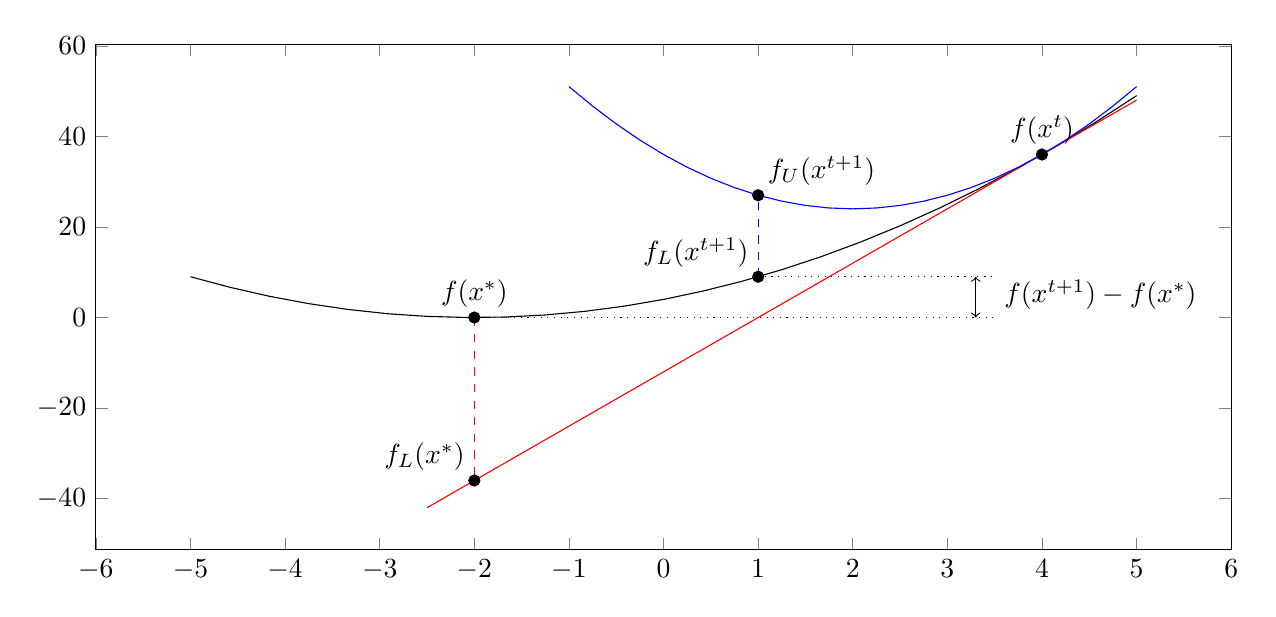
\begin{tikzpicture}
    \begin{axis}[width=16cm,height=8cm]
      \addplot[mark=none] {(x+2)^2};
      \addplot[mark=none,red,domain=-2.5:5] {36+12*(x-4)};
      \addplot[mark=none,blue,domain=-1:5] {36+12*(x-4)+3*(x-4)^2};
      \addplot[only marks] coordinates {
        (4,36) (-2,0) (-2,-36) (1,9) (1,27)
      };
      \node at (axis cs:4,36) [anchor=south] {$f(x^t)$};
      \node at (axis cs:-2,0) [anchor=south] {$f(x^*)$};
      \node at (axis cs:-2,-36) [anchor=south east] {$f_L(x^*)$};
      \node at (axis cs:1,9) [anchor=south east] {$f_L(x^{t+1})$};
      \node at (axis cs:1,27) [anchor=south west] {$f_U(x^{t+1})$};

      \addplot[mark=none,dashed,red] coordinates {
        (-2,0) (-2,-36)
      };
      \addplot[mark=none,dashed,blue] coordinates {
        (1,9) (1,27)
      };

      \addplot[domain=-2:3.5,dotted] {0};
      \addplot[domain=1:3.5,dotted] {9};
      \draw [<->] (axis cs:3.3,0) -- (axis cs:3.3,9);
      \node at (axis cs:3.5,5) [anchor=west] {$f(x^{t+1})-f(x^*)$};
    \end{axis}
  \end{tikzpicture}
  \caption{Illustration of a convex $\beta$-smooth function $f(x)$, with its lower bound $f^L(x)=f
  (x_0)+\langle \nabla f(x_0),x-x_0\rangle$ and upper bound $f^U(x)=f(x_0)+\langle \nabla f(x_0),
  (x-x_0)\rangle + 0.5\beta\|x-x_0\|^2$. The lower bound makes sure $f (x^t)$ is not too far away
  from $f (x^*)$, while
  the upper bound makes sure some progress $f(x^t)-f(x^{t+1})$ are made in each iteration.}
  \label{fig:lower-and-upper-bnd-smooth-cvx}
\end{figure}

\begin{lemma}
  Assume $f:\RR^n\rightarrow \RR$ is $\beta$-smooth, then $\forall x,y\in\RR^n$
  \[
  |f(y)-f(x)- \langle \nabla f(x), y-x\rangle | \leq \frac{\beta}{2}\|y-x\|^2
  \]
\end{lemma}
\begin{proof}
By the fundamental theorem for line integrals,
\[
  f(y) = f(x) + \int_{0}^1 \langle \nabla f(x + t(y-x)), y-x\rangle dt
\]
Plugin $f(y)-f(x)$,
\[
  \begin{aligned}
  |f(y)-f(x)- \langle \nabla f(x), y-x\rangle | \leq \frac{\beta}{2}\|y-x\|^2
  &= \left| \int_0^1 \langle \nabla f(x+t(y-x))-\nabla f(x), y-x\rangle dt \right| \\
  &\leq \|y-x\|\int_0^1 \|\nabla f(x+t(y-x))-\nabla f(x)\| dt \\
  &\leq \|y-x\|\int_0^1 \beta t\|y-x\|dt \\
  &=\frac{\beta}{2}\|y-x\|^2
  \end{aligned}
\]
\end{proof}

If we further know that $f$ is convex, combining the lower bound from the first order condition of
convexity, we get both lower bound and upper bound
\begin{equation}
  0 \leq f(y) - f(x) - \langle \nabla f(x), y-x\rangle \leq \frac{\beta}{2}\|y-x\|^2
  \label{eq:beta-smooth-lower-upper-bnd-0}
\end{equation}
See again Fig.~\ref{fig:lower-and-upper-bnd-smooth-cvx} for an illustration.

\subsection{Convergence Analysis and Tighter Sandwiching}

To analyze the convergence, let $\Delta_t=f(x^t)-f(x^*)$ be the suboptimality gap at $x^t$. Let
$y=x^*$, and $x=x^t$ in \eqref{eq:beta-smooth-lower-upper-bnd-0}, and using the lower bound, we can
upper bound $\Delta_t$ by
\begin{equation}
  \Delta_t = f(x^t)-f(x^*) \leq -\langle \nabla f(x^t), x^*-x^t\rangle
  \leq \|\nabla f(x^t)\|\|x^*-x^t\| \leq R\|\nabla f(x^t)\|
  \label{eq:beta-smooth-grad-analysis-0}
\end{equation}
where we define
\begin{equation}
  R=\max_{1\leq t\leq T}\|x^*-x^t\|
\end{equation}
On the other hand, using the upper bound in \eqref{eq:beta-smooth-lower-upper-bnd-0} by letting
$y=x^{t+1}$ and $x=x^t$, we could lower bound $\Delta_t-\Delta_{t+1}$ by
\begin{equation*}
\begin{aligned}
  \Delta_t-\Delta_{t+1} = f(x^t)-f(x^{t+1})
  &\geq -\langle \nabla f(x^t), x^{t+1}-x^t\rangle - \frac{\beta}{2}\|x^{t+1}-x^t\|^2 \\
  &= \left(\eta_t - \frac{\beta\eta_t^2}{2}\right) \|\nabla f(x^t)\|^2
\end{aligned}
\end{equation*}
Naturally, we want to maximize the lower bound, so the step size is chosen to be
$\eta_t = 1/\beta$. In this case,
\begin{equation}
  \Delta_t - \Delta_{t+1} \geq \frac{1}{2\beta}\|\nabla f(x^t)\|^2
  \label{eq:beta-smooth-grad-analysis-0.5}
\end{equation}
Note \eqref{eq:beta-smooth-grad-analysis-0} and \eqref{eq:beta-smooth-grad-analysis-0.5} are linked
together by $\|\nabla f(x^t)\|$: if $\|\nabla f(x^t)\|$ is large, then moving one step makes a lot
of progress in $\Delta_t-\Delta_{t+1}$; on the other hand, if $\|\nabla f(x^t)\|$ is small,
$\Delta_t$ is also small, meaning we are close to the optimal.
Combining the two equations, we get
\begin{equation}
   \Delta_t - \Delta_{t+1}\geq \frac{1}{2\beta}\|\nabla f(x^t)\|^2
   \geq \frac{1}{2\beta R^2}\Delta_t^2
 \end{equation}
 Note the right hand side is non-negative, so $\Delta_t\geq \Delta_{t+1}$. To solve this recursion,
 divide both side by $\Delta_t\Delta_{t+1}$:
 \begin{equation}
   \frac{1}{\Delta_{t+1}} - \frac{1}{\Delta_t} \geq \frac{1}{2\beta R^2}\frac{\Delta_t}{\Delta_
   {t+1}} \geq \frac{1}{2\beta R^2}
 \end{equation}
 Sum the recursion for $t=2,\ldots,T$, we get
 \[
 \frac{1}{\Delta}_T \geq \frac{T-1}{2\beta R^2} + \frac{1}{\Delta_1}
 \geq \frac{T+3}{2\beta R^2}
 \]
 where the last inequality is because $\Delta_1$ can be controlled by the upper bound in
 \eqref {eq:beta-smooth-lower-upper-bnd-0}. Let $x=x^*$ and $y=x^1$, notice $\nabla f(x^*)=0$,
 \[
 \Delta_1 = f(x^1)-f(x^*) \leq \frac{\beta}{2}\|x^1-x^*\|^2 \leq \frac{\beta R^2}{2}
 \]

At this point, we almost proved Theorem~\ref{thm:beta-smooth}, except that we have to control $R$.
In the following, we will show that $\|x^t-x^*\|$ is actually decreasing at each iteration, and
bound $R$ by $\|x^1-x^*\|$. Recall in the case of subgradient descent, we use the linear lower bound
of the function by the subgradient to construct the inequality in \eqref
{eq:subgrad-lipschitz-analysis-step}. That inequality shows that when $\eta_t$ is small enough,
because the quadratic term decays faster, we get $\|x^{t+1}-x^*\|^2\leq \|x^t-x^*\|^2$. However, in
the case here, since $\eta_t=1/\beta$, especially when $\beta$ is small, we could be moving with
very large step size. So the argument is no longer useful here.

To properly bound $R$, we will need to get a better lower bound of $f$ than in \eqref
{eq:beta-smooth-lower-upper-bnd-0}.
Actually, combining
convexity and $\beta$-smoothness, the lower bound in \eqref{eq:beta-smooth-lower-upper-bnd-0} could
be improved. Consider the extreme case when $f(x)$ is a linear function, then the lower bound is
actually tight. In this case, we also have $\nabla f(x)=\nabla f(y)$. However, if $f(x)$ is not
linear, $\nabla f(x)\neq \nabla f(y)$, we might observe a non-zero gap between $f(x)$ and its linear
lower bound. It is also intuitive that the gap might be larger when the gradient $\nabla f(y)$
changed a lot from $\nabla f(x)$, so we are thinking about getting a better lower bound using the
quantity $\|\nabla f(x)-\nabla f(y)\|$.

\begin{lemma}
  Let $f:\RR^n\rightarrow\RR$ be a convex and $\beta$-smooth function, then $\forall x,y\in\RR^n$
  \begin{equation}
  \frac{1}{2\beta}\|\nabla f(x)-\nabla f(y)\|^2
  \leq f(y) - f(x) - \langle \nabla f(x), y-x\rangle
  \leq \frac {\beta} {2}\|y-x\|^2
  \label{eq:beta-smooth-lower-upper-bnd-1}
  \end{equation}
\end{lemma}
\begin{proof}
  In order to invite both $\nabla f(x)$ and $\nabla f(y)$ into play, we consider a third point
  $z\in\RR^n$, and approximate $f(z)$ from below by $\nabla f(y)$ and from above by $\nabla f(x)$,
  respectively. Using \eqref{eq:beta-smooth-lower-upper-bnd-0}
  \[
  \begin{aligned}
    f(z) - f(x) - \langle \nabla f(x), z-x\rangle &\geq 0\\
    f(z) - f(y) - \langle \nabla f(y), z-y\rangle &\leq \frac{\beta}{2}\|z-y\|^2
  \end{aligned}
  \]
  Multiply the first inequality by $-1$ and sum the two inequalities, we get
  \[
  f(x)-f(y)+\langle \nabla f(x), z-x\rangle - \langle \nabla f(y),z-y\rangle \leq \frac{\beta}
  {2}\|z-y\|^2
  \]
  Re-write the inequality by moving the quantity we want to lower bound to the right,
  \[
   \langle \nabla f(x), z-y\rangle - \langle \nabla f(y),z-y\rangle - \frac{\beta}{2}\|z-y\|^2\leq f
   (y)-f (x)-\langle \nabla f (x),y-x\rangle
  \]
  Inspecting the left hand side, if we let $z=y+\alpha (\nabla f(y)-\nabla f(x))$ for any
  $\alpha\in\RR$, we get
  \[
  \left(\alpha - \frac{\alpha^2\beta}{2}\right)\|\nabla f(y)-\nabla f(x)\|^2\leq f (y)-f (x)-\langle
  \nabla f
  (x),y-x\rangle
  \]
  Since the lower bound is a quadratic function in $\alpha$, we can maximize the lower bound by
  taking $\alpha = 1/\beta$. And the conclusion follows.
\end{proof}

With the improved lower bound of $f$ in \eqref{eq:beta-smooth-lower-upper-bnd-1}, we can now bound
$R$ by showing that
\[
  \begin{aligned}
    \|x^{t+1}-x^*\|^2
    &=\|x^t-x^*\|^2 + \frac{1}{\beta^2}\|\nabla f(x^t)\|^2 - \frac{2}{\beta}\langle \nabla f(x^t),
    x^t-x^*\rangle \\
    &\leq \|x^t-x^*\|^2 + \frac{1}{\beta^2}\|\nabla f(x^t)\|^2
    - \frac{2}{\beta}\left(f(x^t)-f(x^*) + \frac{1}{2\beta}\|\nabla f(x^t)-\nabla f(x^*)\|^2\right)
    \\
    &\leq \|x^t-x^*\|^2 + \frac{1}{\beta^2}\|\nabla f(x^t)\|^2 - \frac{2}{\beta}\times \frac{1}
    {2\beta}\|\nabla f(x^t)\|^2 \\
    & = \|x^t-x^*\|^2
  \end{aligned}
\]
Therefore, $R\leq \|x^1-x^*\|$, which conclude the proof of Theorem~\ref{thm:beta-smooth}.
Actually, in the proof above, we only need a property of the gradient called \emph{co-coercivity}.

\begin{definition}[Co-coercive mapping]
A mapping $F:\RR^n\rightarrow\RR^n$ is co-coercive with parameter $C$ if $\forall x,y\in\RR^d$,
\begin{equation}
  \langle F(x)-F(y), x-y\rangle \geq C\|F(x)-F(y)\|^2
\end{equation}
\end{definition}
By switching the role of $x$ and $y$ in the lower bound of $f$ in \eqref
{eq:beta-smooth-lower-upper-bnd-1}, it is easy to show the following property on the co-coercivity
of $\nabla f(x)$.
\begin{lemma}[Co-coercivity of gradient of convex smooth functions]
Let $f:\RR^n\rightarrow \RR$ be a convex $\beta$-smooth function, then $\nabla f(x)$ is co-coercive
mapping with parameter $1/\beta$. That is
\begin{equation}
  \langle \nabla f(x)-\nabla f(y), x-y\rangle \geq \frac{1}{\beta}\|\nabla f(x)-\nabla f(y)\|^2
\end{equation}
\end{lemma}
We will re-visit some variants of this property in our later adventures of convergence analysis.

\section{Projected Gradient Descent for Convex Smooth Functions with Constraints}

For Problem~\ref{prob:projected-subgradient-descent}, generalization from unconstrained case to
constrained case is straightforward, because we only rely on deriving an upper bound of $\|
(x^t-\eta_tg_t) - x^*\|$, as in \eqref {eq:subgrad-lipschitz-analysis-step}. By the contraction
property of convex projection, as stated in Lemma~\ref{lem:proj-contraction}, we naturally get
\[
  \|\Pi_\sX(x^t-\eta_tg_t)-x^*\| \leq \|(x^t-\eta_tg_t)-x^*\|
\]
and everything follows directly. In the smooth case, things become a bit more complicated.
Especially in the argument that we are making a lot of progress in one step: the contraction might
reduce the aggressive movement we made, and the effective progress might get discounted. So we state
this as a separate problem.

\begin{problem}
  Give a closed convex set $\sX$, and a convex, $\beta$-smooth function $f:\sX\rightarrow \RR$. Find
  a minimizer of $f$ on $\sX$.
\end{problem}

\subsection{Intuition and Convergence Analysis}

In the unconstrained case, we use bound $\Delta_{t+1}=f(x^{t+1})-f(x^*)$ (see Fig.~\ref
{fig:lower-and-upper-bnd-smooth-cvx}) by roughly
\[
\begin{aligned}
  f(x^{t+1})-f(x^*) &= {\color{red}f(x^t)-f(x^*)} - {\color{blue}(f(x^t)-f(x^{t+1}))} \\
  &\leq {\color{red}\langle \nabla f(x^t),x^t-x^*\rangle} - {\color{blue}\frac{1}{2\beta}\|\nabla
  f(x^t)\|^2}
\end{aligned}
\]
where the upper bound of the red term is provided in \eqref{eq:beta-smooth-grad-analysis-0} and the
lower bound of the blue term in \eqref{eq:beta-smooth-grad-analysis-0.5}. And the quantity here is
characterized by $\|\nabla f(x^t)\|$. In the constrained case, we will do a similar thing, but with
a different charactering quantity.

Remember the bounds for both the red term and blue term are directly from \eqref
{eq:beta-smooth-lower-upper-bnd-0}. In the constrained case,
\begin{equation}
  x^{t+1} = \Pi_\sX(x^t-\eta_t \nabla f(x^t))
\end{equation}
By the property of convex projection in Lemma~\ref{lem:proj-contraction}, for any $y\in\sX$,
\[
  \langle x^{t+1} - (x^t-\eta_t\nabla f(x^t)), x^{t+1} - y \rangle \leq 0
  \quad\Leftrightarrow\quad
  \langle \nabla f(x^t), x^{t+1}-y\rangle \leq \frac{1}{\eta_t}\langle x^t-x^{t+1}, x^{t+1}-y\rangle
\]
With this tool, we carry the out the analysis as before, by applying \eqref
{eq:beta-smooth-lower-upper-bnd-0},
\[
  \begin{aligned}
    f(x^{t+1})-f(x^*) &=f(x^t)-f(x^*) - (f(x^t)-f(x^{t+1})) \\
    &\leq \langle \nabla f(x^t),x^t-x^*\rangle + \langle \nabla f(x^t), x^{t+1}-x^t\rangle + \frac
    {\beta}{2}\|x^{t+1}-x^t\|^2 \\
    &= \langle \nabla f(x^t),x^{t+1}-x^*\rangle + \frac{\beta}{2}\|x^{t+1}-x^t\|^2 \\
    &\leq \frac{1}{\eta_t}\langle x^t-x^{t+1}, x^{t+1}-x^*\rangle + \frac{\beta}{2}\|x^{t+1}-x^t\|^2
    \\
    &=\frac{1}{\eta_t}\langle x^t-x^{t+1},x^t-x^*\rangle + \left(\frac{\beta}{2} - \frac{1}
    {\eta_t}\right)\|x^{t+1}-x^t\|^2
   \end{aligned}
\]
In particular, if we still choose the step size $\eta_t=1/\beta$ as in the unconstrained case, we
get
\begin{equation}
\begin{aligned}
  f(x^{t+1})-f(x^*)
  &\leq \langle \beta(x^t-x^{t+1}), x^t-x^*\rangle - \frac{\beta}{2}\|x^ {t+1}-x^t\|^2 \\
  &= \langle g_\sX(x^t), x^t-x^*\rangle - \frac{1}{2\beta}\|g_\sX(x^t)\|^2
  \label{eq:constrained-beta-smooth-3-point}
\end{aligned}
\end{equation}
where we have defined the quantity
\begin{equation}
  g_\sX(x^t) = \beta(x^t-x^{t+1})
\end{equation}
Note in the unconstrained case, $\beta (x^t-x^{t+1})=\nabla f(x^t)$, and its norm characterized our
bounds. It turns out that in the constrained case, this quantity plays the same role. Actually, the
derivation above does not use the optimality of $x^*$, so replacing $x^*$ with any $y\in\sX$, we get
the following lemma.

\begin{lemma}[Three-point Inequality]
Let $x,y\in\sX$ and $x^+=\Pi_\sX\left(x-\frac{1}{\beta}\nabla f(x)\right)$, and $g_\sX(x)=\beta
(x-x^+)$. Then
\begin{equation}
  f(x^+)-f(y) \leq \langle g_\sX(x), x-y\rangle - \frac{1}{2\beta}\|g_\sX(x)\|^2
\end{equation}
\end{lemma}

By plugging in $x=x^t$, $y=x^*$, we immediately get the upper bound
\begin{equation}
  \Delta_{t+1} = f(x^{t+1})-f(x^*) \leq \langle g_\sX(x^t),x^t-x^*\rangle
  \leq \|g_\sX(x^t)\|\|x^t-x^*\|
\end{equation}
Similarly, plugging in $x=y=x^t$, we get the lower bound
\begin{equation}
\Delta_t - \Delta_{t+1} = f(x^t)-f(x^{t+1}) \geq \frac{1}{2\beta}\|g_\sX(x^t)\|^2
\end{equation}
The two inequalities are now linked by $\|g_\sX(x^t)\|$, combing them, we get
\[
  \Delta_t - \Delta_{t+1} \geq \frac{1}{2\beta} \frac{\Delta_{t+1}^2}{\|x^t-x^*\|^2}
  \geq \frac{\Delta_{t+1}^2}{2\beta R^2}
\]
where again we let $R=\max_{1\leq t\leq T}\|x^t-x^*\|$.


\bibliography{references}

\end{document}
